% !TEX root = ../TechProject.tex

\graphicspath{{Chapter6/}}

\chapter{Results and Discussion}

This chapter will provide analysis and discussion of the results from the experiment described
in Chapter 5. The experiment sought to answer the question presented in Chapter 4.
\\
\\
\textit{Is the proposed method a suitable solution to automate recommendations of songs suitable for adding to a given DJ set?}.
\\
\\
Chapter 6.1 will present the appropriate latent factors to use on the dataset. And then to see how varying the input DJ Set tracklist lengths could also improve reccomended songs.

\subsection{R-Precision Values}
\begin{center}
	\begin{tabular}{ | m{3cm}| m{3cm} | } 
		\hline
		Latent Factors & R-Precision\\ 
		\hline
		100 &	0.1063612311\\
		\hline
		90 &	0.1198826892\\
		\hline
		80	&	0.1198826892\\
		\hline
		70	&	0.1206836885\\
		\hline
		60	&	0.1119354921\\
	\end{tabular}
\end{center}

The following controlled variable was the list of dj sets and the independent variable was the latent factors for making the Alternating Least Squared model. This was used to decipher what parameter value for latent factors was gonna produce the most accurate recommendations. It didn't want to be so big that the recommendations were "over-fitting", or too low if the recommendations were too random. In the medium article, Chow used 50 latent factors \citep{chow_music_2020}. This was used as a reference point to make the range from 20 - 100 latent factors to experiment on.
\begin{figure}[H]
	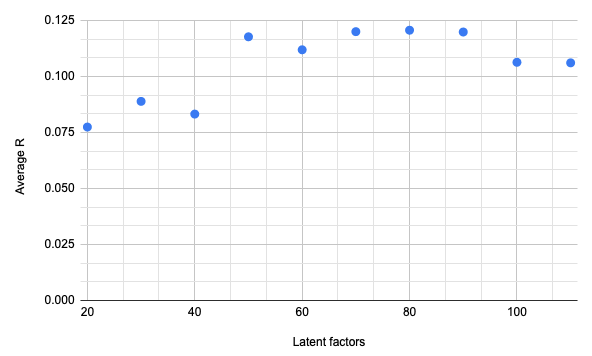
\includegraphics[scale=0.6]{images/average_r_over_latent}
	\centering
	\caption{Scatter graph of average r-precision values with different latent factors} 
\end{figure}

The results indicate the performance of alternating least squares (ALS) algorithm in recommending items based on different number of latent factors. The average r-precision, a measure of the relevancy of recommended items to the user, was used to evaluate the algorithm's effectiveness across different latent factors.

The analysis shows that the performance of the application varies significantly with the number of latent factors used. The highest average r-precision of 0.1207 was obtained when 70 latent factors were used, while the lowest value of 0.0774 was obtained when only 20 latent factors were used. However, the performance of the algorithm was not monotonically increasing or decreasing with the number of latent factors. For instance, there was a slight increase in average r-precision from 50 to 80 latent factors, but a decrease from 70 to 60 latent factors.

The results suggest that selecting an appropriate number of latent factors is crucial for the performance of ALS algorithm. Using too few latent factors can lead to poor recommendations, while using too many can lead to overfitting and poor generalization. Therefore, it is important to strike a balance between the number of latent factors and the algorithm's performance. Overall, the study provides insights into the performance of ALS algorithm with varying number of latent factors and highlights the importance of selecting the optimal number of factors for effective recommendation.


% note that \Blindocument has 5 numbered levels, despite setting secnumdepth above. I (and many style guides) would suggest using no more than 3 numbered levels (incl. the chapter), with the option of a fourth unnumbered level.